\chapter*{Appendix A: Physical Experimental Setup and Printable Layout Artifacts}
\label{ch:appendix_physical_setup}

\section*{A.1 Overview of the Physical Setup}
\label{sec:appendix_setup_overview}
The following Appendix demonstrates the physical layout of the experiment, including the files to print for use in this study. The whole system only requires a regular RGB camera, one piece of ordinary printed paper, and a flat surface, without any other specialized equipment such as depth cameras or sensor gloves.

The physical setup of the desk is shown in Figure~\ref{fig:appendix_physical_setup}. A cheap USB webcam is attached to an adjustable desk arm over the workspace. In the physical experiment, the height $h$ of the camera above the desktop surface can vary between $14\text{ cm}$ and $28\text{ cm}$, and the horizontal distance $d$ between the base of the camera mount to the paper layout can vary between $14\text{ cm}$ and $28\text{ cm}$.

The downward viewing angle of the camera does not require any manual calculation, as it can be derived by employing right-angle trigonometry on the physical parameters:
\begin{equation}
\theta = \arctan\left(\frac{h}{d}\right)
\label{eq:appendix_camera_tilt_trig}
\end{equation}
The analysis of the trigonometric expression for the operating range of values gives:
\begin{itemize}
    \item \textbf{Minimum downward angle (lowest height and furthest distance):} For $h = 14\text{ cm}$ and $d = 28\text{ cm}$:
    \begin{equation}
    \theta_{\min} = \arctan\left(\frac{14}{28}\right) = \arctan(0.5000) \approx 26.6^\circ
    \end{equation}
    \item \textbf{Maximum downward angle (highest height and closest distance):} For $h = 28\text{ cm}$ and $d = 14\text{ cm}$:
    \begin{equation}
    \theta_{\max} = \arctan\left(\frac{28}{14}\right) = \arctan(2.0000) \approx 63.4^\circ
    \end{equation}
\end{itemize}
This provides the pitch angle downwards in the range of $26.6^\circ$ to $63.4^\circ$ with respect to the horizontal plane of the desk surface (or equivalently, the perspective angle of $26.6^\circ$ to $63.4^\circ$ with respect to the normal of the surface). The direct line-of-sight Euclidean distance $R = \sqrt{h^2 + d^2}$ spans from $\sqrt{14^2 + 14^2} \approx 19.8\text{ cm} \approx 20\text{ cm}$ (minimum) to $\sqrt{28^2 + 28^2} \approx 39.6\text{ cm} \approx 40\text{ cm}$ (maximum). The flat layout of the printed paper keyboard is positioned on the table surface and the four AprilTag fiducials at the borders are clearly visible to the camera during single-handed interaction.

\begin{figure}[htbp]
\centering
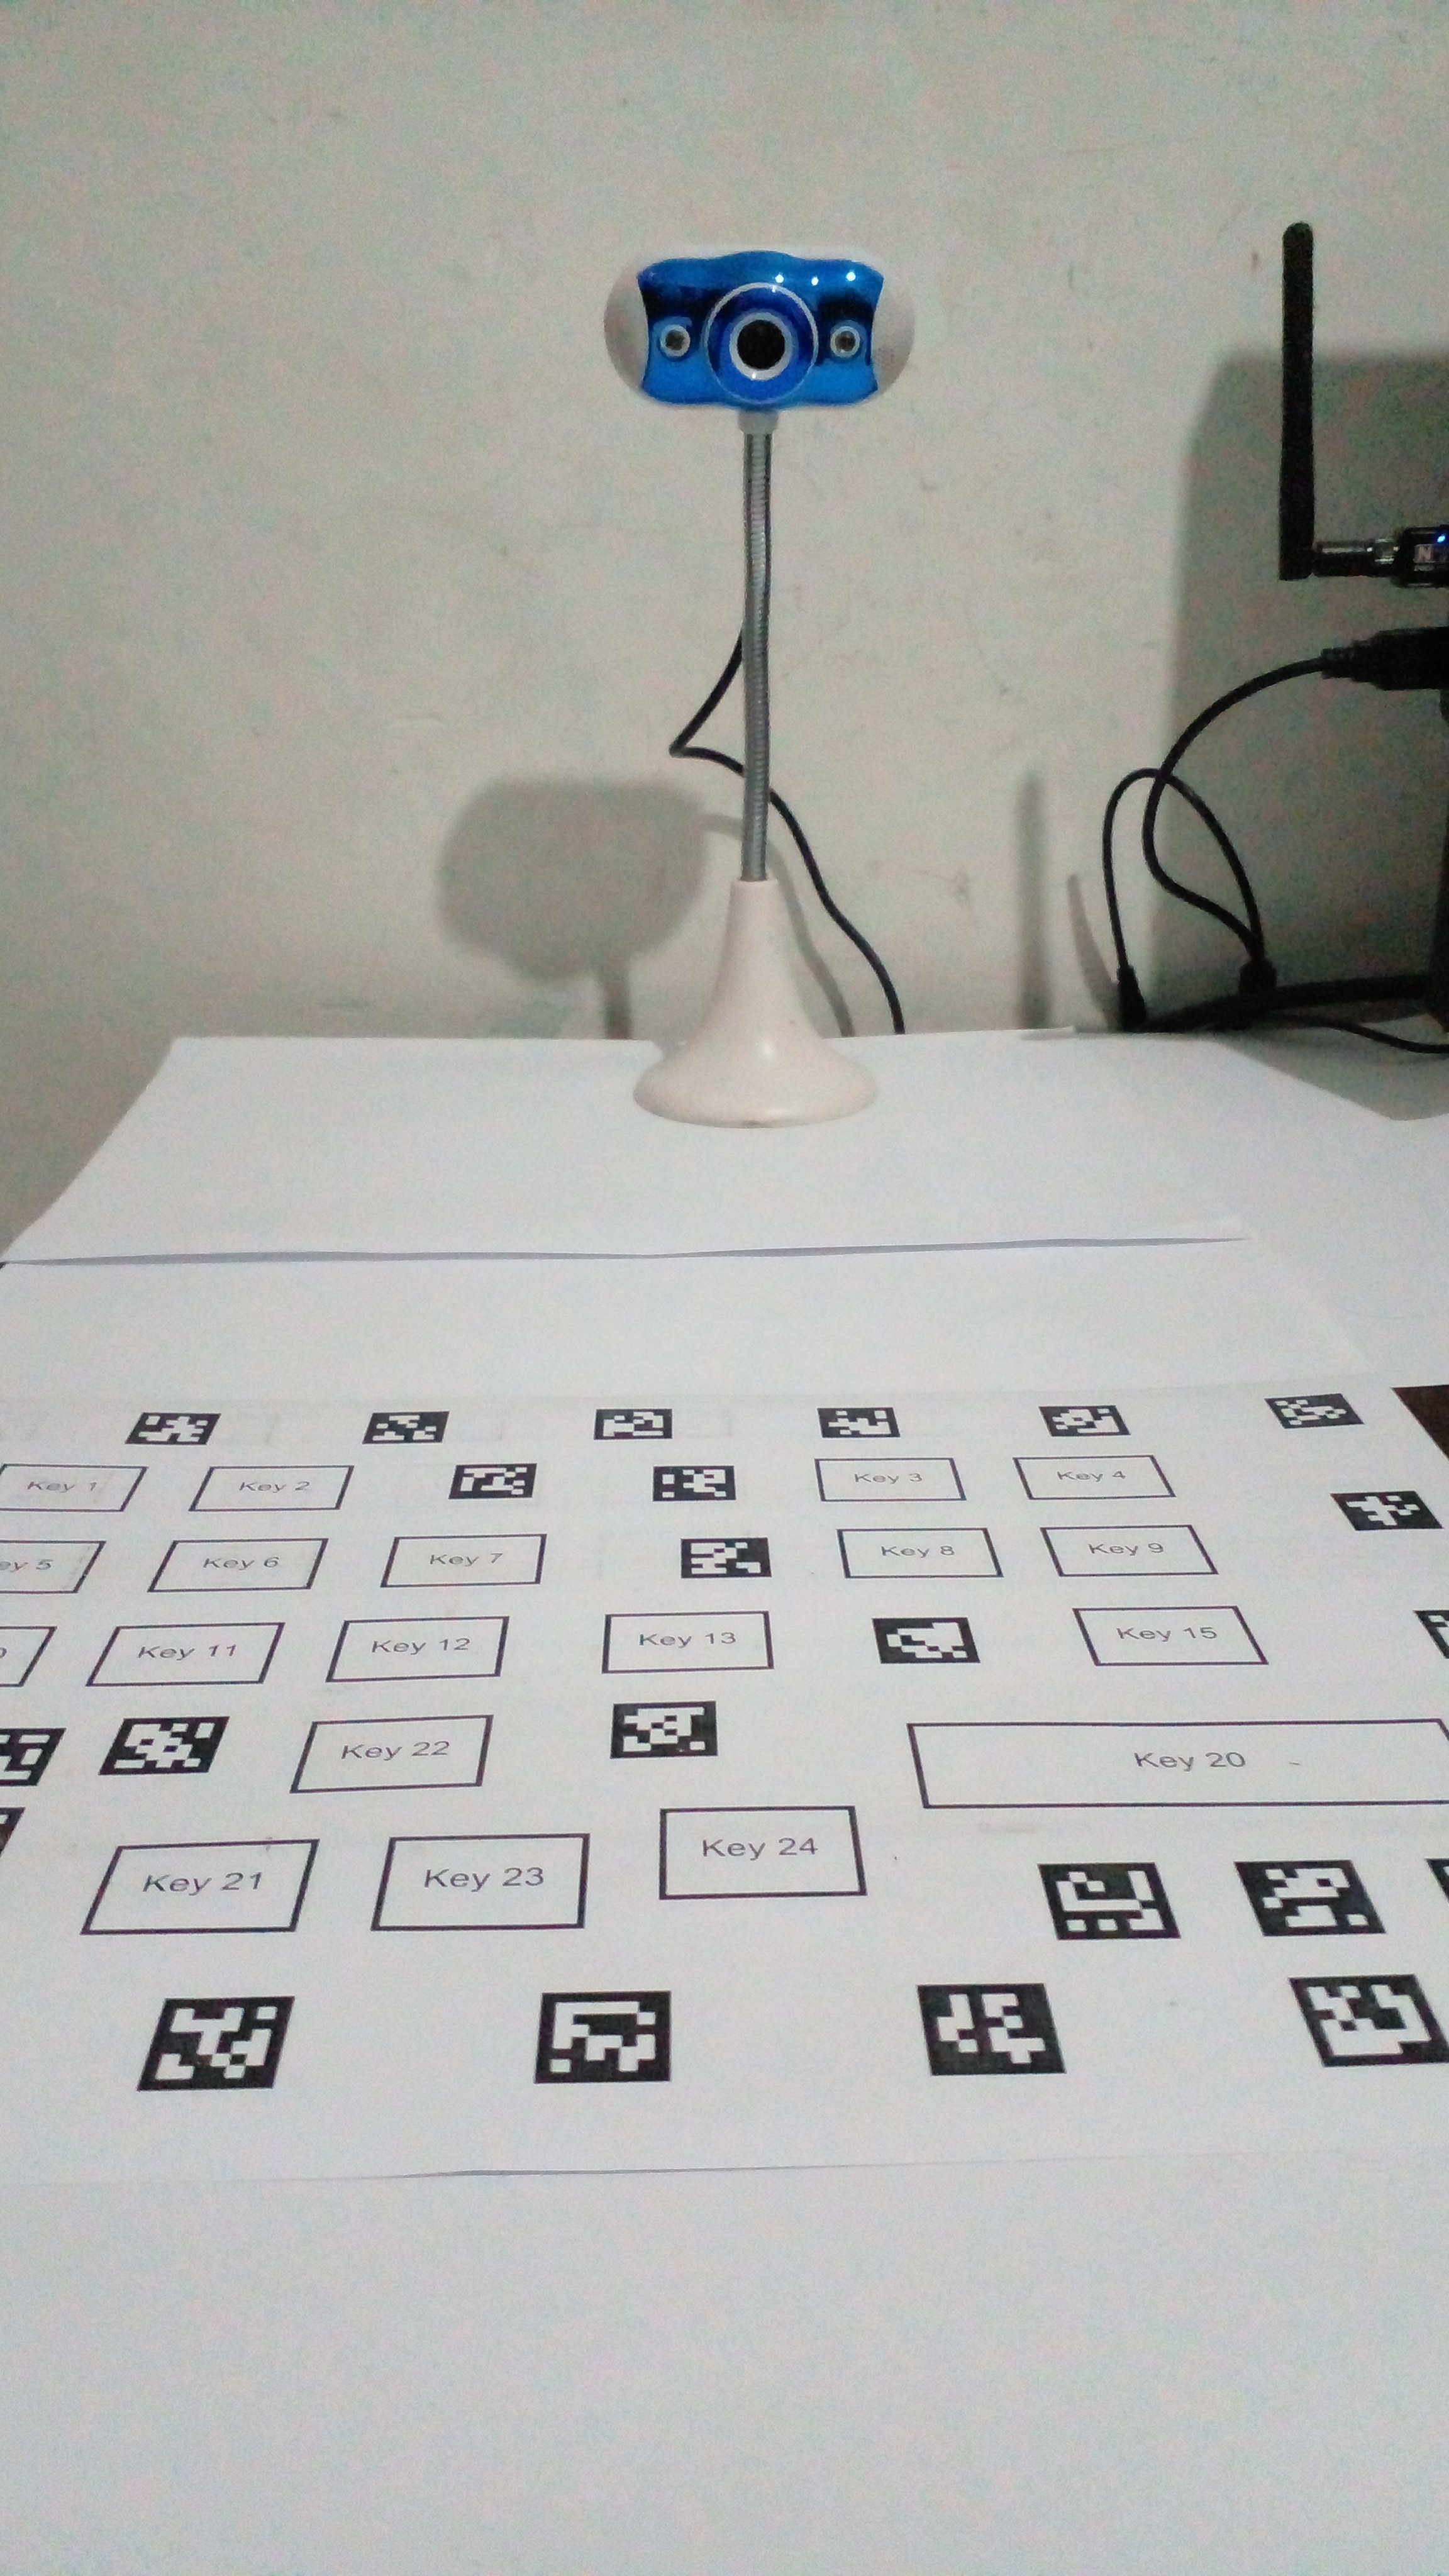
\includegraphics[width=0.72\textwidth]{figures/physical_setup_image_upright.jpg}
\caption{Physical experimental desk setup with monocular USB webcam mounted on an adjustable arm above the printed paper macro keyboard layout.}
\label{fig:appendix_physical_setup}
\end{figure}

\newpage

\section*{A.2 Printable Vector Layout Artifact}
\label{sec:appendix_printable_layout}
The design of the layout that was generated using Application~1 (Layout Designer) is shown in Figure~\ref{fig:appendix_printable_pdf}. The design has been saved at 300~DPI, allowing it to be easily printed in high resolution on ordinary A4 paper using an ordinary office printer. Four AprilTags with IDs 0, 1, 2, and 3 have been located in the corners. The central part contains the custom macro keys with clear border lines and button names.

\begin{figure}[htbp]
\centering
\includegraphics[width=0.88\textwidth]{figures/printable_layotu_pdf_image.png}
\caption{Exported 300~DPI vector PDF layout embedded with AprilTag border fiducials ready for standard desktop paper printing.}
\label{fig:appendix_printable_pdf}
\end{figure}
